\section{Collaborazione uomo-robot}

La robotica industriale ha assunto un ruolo sempre più rilevante nei moderni processi produttivi, grazie alla possibilità di automatizzare attività ripetitive, incrementare la produttività e garantire elevati livelli di precisione e ripetibilità. Tradizionalmente, l'impiego di robot industriali è stato caratterizzato dalla separazione fisica tra l'area di lavoro dell'operatore e quella del robot, mediante l'utilizzo di barriere, recinzioni o altri dispositivi volti a impedire l'accesso dell'uomo alla zona operativa durante il movimento del robot.
Questo approccio permette di ridurre il rischio di interazione accidentale, separando nettamente le attività svolte dall'uomo e quelle affidate al sistema robotico. Tale separazione, tuttavia, può risultare poco conveniente in applicazioni nelle quali le capacità del lavoratore e quelle del robot possono essere integrate per ottenere un processo più efficiente e flessibile.

Da questa esigenza nasce il concetto di collaborazione uomo-robot, nel quale l'operatore umano e la macchina robotica operano all'interno di uno spazio condiviso, come schematizzato in Figura \ref{fig:collaborazione}, e possono contribuire simultaneamente alla realizzazione di uno stesso compito \cite{BARATTA20231887}. In questo contesto, il robot non viene più considerato come un sistema autonomo e separato dall'operatore, ma come uno strumento in grado di interagire con esso e di supportarne le attività. La condivisione dello spazio di lavoro permette quindi di combinare le caratteristiche complementari dell'uomo e del robot, con l'obiettivo di ottenere sistemi produttivi più flessibili e adattabili rispetto alle soluzioni di automazione tradizionali.

\begin{figure}[htbp]
    \centering
    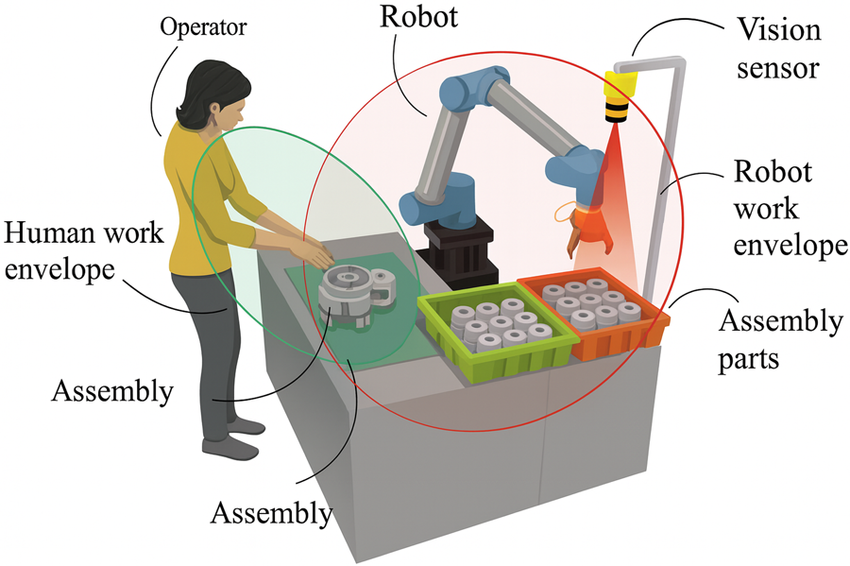
\includegraphics[width=0.8\linewidth]{figure_tesi/Application-of-cobots-in-the-manufacturing-process.png}
    \caption{Rappresentazione schematica di una cella di lavoro collaborativa. Viene evidenziata la sovrapposizione tra il volume operativo dell'operatore (\textit{Human work envelope}) e l'area di lavoro del robot (\textit{Robot work envelope}).}
    \label{fig:collaborazione}
\end{figure}

Le applicazioni della collaborazione uomo-robot sono principalmente legate a situazioni nelle quali le capacità dell'operatore e quelle del robot risultano complementari \cite{Montini2024}. Il robot può, ad esempio, occuparsi di attività caratterizzate da elevata ripetibilità, precisione o movimentazione di carichi, mentre l'operatore può intervenire nelle operazioni che richiedono capacità decisionali, adattamento a condizioni variabili o manipolazioni più complesse. Questa suddivisione delle attività permette di sfruttare i vantaggi dell'automazione mantenendo, allo stesso tempo, la flessibilità e la capacità di adattamento proprie dell'operatore umano.

La collaborazione diretta tra uomo e robot può quindi trovare applicazione in diversi processi industriali, tra cui assemblaggio, movimentazione, manipolazione e attività di supporto all'operatore. In questi scenari, la possibilità di lavorare all'interno dello stesso spazio consente di ridurre la necessità di separare fisicamente le due attività e di progettare processi nei quali uomo e robot possano intervenire in maniera complementare sullo stesso task.

La condivisione dello spazio di lavoro introduce tuttavia una problematica fondamentale: la necessità di garantire condizioni di sicurezza durante l'interazione. A differenza delle applicazioni tradizionali, nelle quali la presenza dell'operatore nella zona di movimento del robot viene impedita, nei sistemi collaborativi la presenza umana deve essere considerata come una condizione normale di funzionamento. La gestione della sicurezza assume quindi un ruolo centrale nella progettazione di questi sistemi e rappresenta uno degli aspetti fondamentali per consentire una collaborazione efficace tra uomo e robot.

\section{Sicurezza nella collaborazione uomo-robot}

La possibilità di condividere lo spazio di lavoro tra operatore umano e robot introduce la necessità di adottare specifiche strategie volte a garantire la sicurezza dell'interazione \cite{Li2024}. Il rischio associato alla collaborazione dipende infatti da diversi fattori, tra cui la geometria del robot, la velocità di movimento, le caratteristiche dell'ambiente di lavoro e la posizione dell'operatore rispetto al sistema robotico.

Un primo elemento che può contribuire alla riduzione delle conseguenze di un eventuale contatto è rappresentato dalla progettazione del robot. La geometria e i materiali utilizzati per la realizzazione dei componenti che possono entrare in contatto con l'operatore possono infatti influenzare le conseguenze di una collisione. In particolare, l'impiego di superfici arrotondate e l'assenza di spigoli vivi permettono di ridurre la possibilità che un eventuale contatto provochi lesioni all'operatore. Sebbene questi accorgimenti contribuiscano alla sicurezza del sistema, essi non sono sufficienti a garantire autonomamente condizioni di sicurezza durante l'interazione.

La sicurezza dei sistemi robotici collaborativi è pertanto regolamentata da specifici standard internazionali, che definiscono principi e requisiti per la progettazione e la valutazione delle applicazioni di collaborazione uomo-robot \cite{ISO15066}. Tra gli aspetti considerati rientrano anche le condizioni che devono essere rispettate affinché l'operatore possa condividere lo spazio di lavoro con il robot in condizioni di sicurezza.

Un aspetto particolarmente rilevante è rappresentato dalla distanza tra l'operatore e il robot. Durante il movimento, infatti, è necessario che il sistema sia in grado di rilevare una situazione potenzialmente pericolosa con sufficiente anticipo da permettere l'adozione di un'azione correttiva prima che si verifichi un contatto. La distanza necessaria non può quindi essere considerata come un valore fisso, ma deve essere valutata tenendo conto della dinamica del sistema e, in particolare, della velocità del robot e dell'operatore e dei tempi necessari affinché il sistema possa reagire alla situazione di rischio \cite{Marvel2017}.

Un approccio alla gestione di questo problema è rappresentato dallo \textit{Speed and Separation Monitoring} (SSM), nel quale la distanza tra l'operatore e il robot viene monitorata durante l'esecuzione del task. Con riferimento alla Figura \ref{fig:SSM}, quando la separazione tra i due è tale da non garantire più le condizioni di sicurezza, il sistema può intervenire modificando il comportamento del robot, ad esempio riducendone la velocità (zona gialla) o arrestandone il movimento (zona rossa). La distanza necessaria per garantire la sicurezza dipende quindi dalle condizioni di funzionamento del sistema e deve essere valutata considerando anche il tempo necessario affinché il robot possa effettuare l'azione prevista.

\begin{figure}
    \centering
    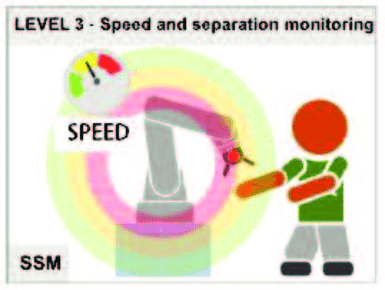
\includegraphics[width=0.5\linewidth]{figure_tesi/Speed-and-separation-monitoringVillani-et-al-2018.png}
    \caption{Rappresentazione schematica del principio di Speed and Separation Monitoring (SSM).}
    \label{fig:SSM}
\end{figure}

Nell'ambito dello SSM sono state sviluppate diverse strategie finalizzate a migliorare il compromesso tra sicurezza e continuità operativa. Un arresto del robot ogni volta che l'operatore si avvicina alla zona di lavoro permette di adottare un comportamento conservativo, ma può comportare frequenti interruzioni dell'attività e conseguenti riduzioni della produttività. Per questo motivo, sono state studiate strategie che permettono di adattare dinamicamente le condizioni di sicurezza in funzione del movimento del robot e dell'operatore. In particolare, Scalera et al. \cite{Scalera2022} propongono una strategia basata sullo scaling online delle zone di sicurezza dinamiche, con l'obiettivo di migliorare la fluidità e la produttività della collaborazione mantenendo le condizioni di sicurezza.

Il presente lavoro si inserisce in questo contesto e si concentra sul confronto tra due differenti strategie software per la gestione di una possibile situazione di collisione. Le due procedure utilizzano le informazioni relative alla posizione dell'operatore e al movimento del robot per valutare le condizioni di sicurezza, ma adottano strategie differenti per la gestione del movimento. La prima procedura prevede l'arresto del robot quando viene prevista una possibile collisione, mentre la seconda modifica il movimento del robot con l'obiettivo di mantenere una distanza di sicurezza dall'operatore senza ricorrere necessariamente all'arresto completo.

\section{Obiettivo della tesi}

L'obiettivo del presente lavoro di tesi è quello di sviluppare e analizzare due strategie di controllo per la collaborazione sicura uomo-robot, entrambe basate sull'utilizzo della visione artificiale per il rilevamento della presenza e della posizione dell'operatore all'interno dello spazio di lavoro del robot.

La prima strategia, arresto forzato, deriva dagli studi di Scalera et al. \cite{Scalera2022}, che hanno analizzato l'impiego di capsule di ingombro dinamiche, chiamate \textit{Sphere Swept Lines} o SSL, secondo il paradigma di \textit{Speed and Separation Monitoring} o SSM. In particolare viene calcolato il tempo minimo di arresto del robot in funzioni di vari vincoli del robot. 
La seconda strategia estende il primo approccio introducendo una tecnica di modifica del movimento del robot basato su un controllo di ammettenza \cite{Qyrani2026}. In questo modo il robot mantiene una distanza di sicurezza modificando la propria traiettoria, evitando se possibile l'arresto completo del robot.
Il confronto viene effettuato attraverso le seguenti metriche:
\begin{itemize}
    \item durata complessiva di esecuzione del task
    \item tempo durante il quale il robot è fermo
    \item numero di arresti
    \item tempo durante il quale operatore e robot risultano contemporaneamente attivi all'interno dello spazio di lavoro
\end{itemize}

Lo studio mira quindi a determinare le caratteristiche e le prestazioni delle due strategie e ad evidenziarne vantaggi e limiti in relazione all'impiego in scenari di collaborazione uomo-robot.

\section{Struttura della tesi}

La tesi è organizzata in cinque capitoli che descrivono il processo di riconoscimento del problema, implementazione di una soluzione e confronto tra i due approcci software.

Il primo capitolo introduce il contesto della collaborazione uomo-robot, descrivendo le principali problematiche legate alla sicurezza dell'interazione e presentando gli obiettivi del lavoro.

Nel secondo capitolo vengono descritti i due approcci proposti per la gestione della sicurezza. Per ciascuna procedura vengono illustrati il principio d funzionamento, le grandezze considerate e la strategia adottata per la gestione del movimento del robot.

Il terzo capitolo è dedicato all'implementazione sperimentale. Vengono presentati il sistema robotico utilizzato, l'ambiente di sviluppo, l'implementazione delle due procedure e la configurazione degli esperimenti. Vengono inoltre definite le metriche utilizzate per il confronto e il protocollo sperimentale adottato.

Nel quarto capitolo vengono presentati e discussi i risultati ottenuti durante la fase sperimentale. Le due procedure vengono confrontate sulla base delle metriche definite, analizzandone il comportamento in termini di sicurezza, continuità operativa ed efficienza nell'esecuzione del task.

Il quinto capitolo, infine, riassume i principali risultati del lavoro e presenta le conclusioni dello studio, evidenziando vantaggi e limiti delle due stratege utilizzate e indicando possibili sviluppi futuri.